% Preamble
% Compile with XeLateX

\documentclass[11 pt,oneside,a4paper,titlepage]{article}
\usepackage{preamble}
\graphicspath{{PIC/}}
%%%%%%%%%%%%%%%%%%%%%%%%%%%%%%%%%%%%%%%%%%%%%%%%%%%%%%%%%%%%%%%%%%%%%%%%%%%%%%%%%%%%%%
\begin{document}

\sidebar{sideBarColor!25}
\simpleheader{titleBackColor}{Riccardo}{Periotto}{Computer Scientist |  Autonomous Systems Engineer}{white}

% Start Minipages
\vspace*{3.49cm}% start 8 cm from the top of the page}
    \adjustbox{valign=t}{\begin{minipage}{7.3cm} % large 7.4 cm from the top
    \vspace*{1.2cm} % text starts 1cm under the top of the minipage
            
        % Picture
        \begin{center}
        \begin{tikzpicture}
            \node[
            circle,
            minimum size=\cvPictureWidth,
            path picture={
            \node at (path picture bounding box.center){
             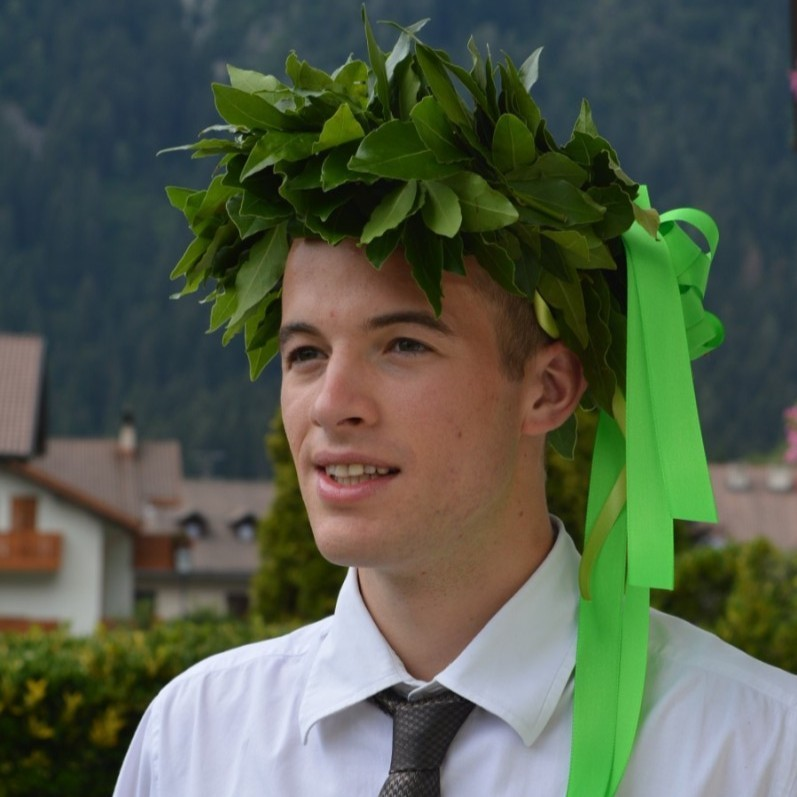
\includegraphics[width=\cvPictureWidth]{Profile.jpg}
             };
             }]
            {};
        \end{tikzpicture}
        \end{center}

        %%%%%%%%%%%%%%%%%%%%%%%%%%%%%%%%%%%%%%%%%%%%%%%%%%%%
        % Profile section
        \ruleline{\textbf{About me}}
        Guided by my passion for studying and technology, I approached the world of ICT in high school and delved into the subject until I graduated in Trento. Between my bachelor’s and master’s degrees, I worked in the field to understand what my passion really was. I am now in the final year of my master’s degree in autonomous systems and my main goal is to develop software for robots. Industrial
        robotics, control, and deep learning are the subjects I prefer and I am ready to apply them to my next challenge!
        %%%%%%%%%%%%%%%%%%%%%%%%%%%%%%%%%%%%%%%%%%%%%%%%%%%
        % Contact Section
        \ruleline{\textbf{Contact}}
        \begin{tikzpicture}[every node/.style={inner sep=0pt, outer sep=0pt}]
        \matrix [
        column 1/.style={anchor=center,contactIcon},
        column 2/.style={anchor=west,align=left,contactIcon},
        column sep=5pt,
        row sep=5pt] (contact) {
        \node{\faMale};
         & \node{Born on 15/09/1998, Age 24};\\
        \node{\faEnvelope}; 
         & \node{\href{mailto:riccardo.periotto@gmail.com}{riccardo.periotto@gmail.com}};\\
        \node{\faPhone}; 
         & \node{+39 3662570766};\\ 
        \node{\faMapMarker}; 
        & \node{Teknikringen 68A \\ 114 28 Stockholm, Sweden};\\
        \node{\faLinkedinSquare}; 
        & \node{\href{https://www.linkedin.com/in/riccardo-periotto/}{riccardo-periotto}};\\
        \node{\faGithubSquare}; 
        & \node{\href{https://github.com/riccardoperiotto}{riccardoperiotto}};\\
        \node{\faCar};
        & \node{Driving License B};\\
        };
        \end{tikzpicture} 
        
        %%%%%%%%%%%%%%%%%%%%%%%%%%%%%%%%%%%%%%%%%%%%%%%%%%%
        % Languages
        \ruleline{\textbf{Languages}}
        \begin{tikzpicture}[every node/.style={inner sep=0pt, outer sep=0pt}]
        \matrix [
        column 1/.style={anchor=center,contactIcon},
        column 2/.style={anchor=west,align=left,contactIcon},
        column sep=5pt,
        row sep=5pt] (contact) {
        \node{\flag{Italy.png}};
        & \node{Italian - Native Language};\\
        \node{\flag{England.png}};
        & \node{English - Professional Knowledge};\\
        \node{\flag{German.png}};
        & \node{German - Basic Knowledge};\\
        };
        \end{tikzpicture} 
        
        %%%%%%%%%%%%%%%%%%%%%%%%%%%%%%%%%%%%%%%%%%%%%%%%%%%%
        % Programming Languages 
        \ruleline{\textbf{Programming languages}}
        \begin{center}
            \cvtag{C\#}\cvtag{C/C++}\cvtag{Python}\cvtag{Javascript}\cvtag{Maple}\cvtag{MATLAB}\cvtag{R}\cvtag{Java}
        \end{center}
        
        %%%%%%%%%%%%%%%%%%%%%%%%%%%%%%%%%%%%%%%%%%%%%%%%%%%%
        % Professional skills 
        \ruleline{\textbf{Professional skills}}
        \begin{center}
            \cvtag{Control}\cvtag{Machine Learning}\cvtag{Model Predictive Control}\cvtag{Deep Learning}\cvtag{Industrial Robotics}\cvtag{Mechatronics}\cvtag{Algorithms}\cvtag{Data Structure}\cvtag{Programming}\cvtag{Software Engineering}\cvtag{Database}\cvtag{Modeling}\cvtag{Operating Systems}\cvtag{Full Stack Development}
        \end{center}
    \end{minipage}} %
    \hfill 
%%%%%%%%%%%%%%%%%%%%%%%%%%%%%%%%%%%%%%%%%%%%%%%%%%%%%%%%%
%%%%% MAIN SECTION %%%%%%%%%%%%%%%%%%%%
    \adjustbox{valign=t}{\begin{minipage}{11.3cm}
        \vspace*{1cm}
        \section*{{\faGraduationCap} EDUCATION}

        \vspace*{0.22cm}
            
        \MySection{sep 2022-\\ Ongoing}{kth.png}{Master's Degree}{KTH Royal Institute of Technology}{Stockholm, Sweden}{Autonomous System\\}{Second year of the Master's degree in Autonomous System, EIT Digital program}
    
        \vspace*{0.22cm}

        \MySection{jul 2017-\\aug 2020}{tum.png}{Summer School}{Technical University of Munich}{Munich, Germany}{Industry 4.0\\}{EIT Digital program Summer School. Topic: IoT platforms for Industry 4.0}
        
        \vspace*{0.22cm}

        \MySection{sep 2017-\\jul 2020}{unitn.jpg}{Master's Degree}{University of Trento}{Trento, Italia}{Autonomous System\\}{First year of the Master's degree in Autonomous System, EIT Digital program}
        
        \vspace*{0.22cm}
        
        \MySection{sep 2021-\\sep 2023}{}{Master's Degree}{EIT Digital}{Europe}{Autonomous Systems}
            
        \vspace*{0.22cm}
            
        \MySection{sep 2017-\\jul 2020}{}{Bachelor's Degree}{University of Trento}{Trento, Italia}{Computer Science\\}{\textbf{Degree: 110/110 with honours}}
        
        \vspace*{0.22cm}
            
        \MySection{sep 2014-\\jul 2017}{}{High School Diploma}{ITT Marconi Rovereto Marconi}{Rovereto, Italia}{Computer Science\\}{\textbf{Grade: 100/100 with honours}}
        
        %%%%%%%%%%%%%%%%%%%%%%%%%%%%%%%%%%%%%%%%%%%%%%%%%%%
        % Work Experience
        \section*{{\faSuitcase} WORK EXPERIENCE IN THE STUDY SECTOR}
            
        \MySection{jan 2021-\\jul 2021}{Polytec.jpg}{Software Engineer}{BM Group Polytec S.p.A.}{Borgo Chiese, Italy}{Software engineering and manufacturing\\}{Development of cloud solution for industrial plants and robotic cells} 
            
        \vspace*{0.22cm}
        
        \MySection{nov 2020-\\dec 2020}{}{Data Engineer}{Capgemini}{Milan, Italy}{}{Think fast: this was not my job} 
        \vspace*{0.22cm}
          
        \MySection{oct 2019-\\feb 2020}{}{Computer Science Intern}{SpazioDati S.r.l.}{Trento, Italy}{}{Thesis project with large datasets and company APIs}  
        
        %%%%%%%%%%%%%%%%%%%%%%%%%%%%%%%%%%%%%%%%%%%%%%%%%%%
        % Information Technology Skills
        \section*{{\faDesktop} FRAMEWORKS AND TOOLS (main ones)}
        
        \ITCcompetence{Software development}{
        \textbf{.NET}: \textit{advanced}\\
        \textbf{Node.js}: \textit{advanced}\\
        \textbf{Unity}: \textit{intermediate}\\
        }
        
         \ITCcompetence{ML/DL}{
        \textbf{Scikit-learn}: \textit{intermediate}\\
        \textbf{PyTorch}: \textit{intermediate}\\
        }
        
        \ITCcompetence{Others}{
        \textbf{git}: \textit{advanced}\\
        \textbf{ROS2}: \textit{beginner}\\
        \textbf{MapleSim}: \textit{beginner}\\
        }
        
        \vspace*{0.22cm}
        
        Updated version of this document available at: \href{https://riccardoperiotto.github.io/CurriculumVitae/CV-RiccardoPeriotto.pdf}{CV-RiccardoPeriotto}. \\
        Date: \today.
    \end{minipage}} %
\end{document}
